\chapter{Analysis}
\section{Introduction}
This chapter will present the analysis of the 2 systems presented in Chapter 6 and 7. Also we will take the better system according to our needs and present the modified system according to our system.
\section{OpenID Based pseudonym System}
\begin{figure}[h]
	\centering
	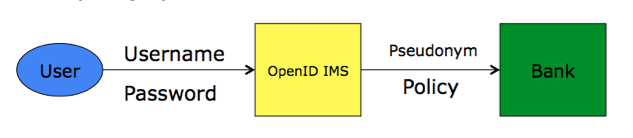
\includegraphics[width=\textwidth]{figures/OpenID}
	\caption{Pseudonym System with OpenID IMS}
	\label{fig:OpenID}
\end{figure}
With the use of OpenID IMS we add a pseudonymous layer in the system. This provides us the necessary privacy. But in order to do so OpenID provider needs access to a lot of data. Some of the example data is:
\begin{itemize}
\item UserID
\item Account ID 
\item Policies	
\end{itemize}
In addition to that, the provider needs to store the mapping database from UserID to Pseudonym. Bank really has to trust the provider with storage of all this sensitive data. In some cases bank might not want the provider to store such data by themselves.
\\In case there is a discrepancy, the authorities need to go both to the bank to get the transaction data as well as the provider for the mapping data.
\section{IDEMIX Based pseudonym System}
\begin{figure}[h]
	\centering
	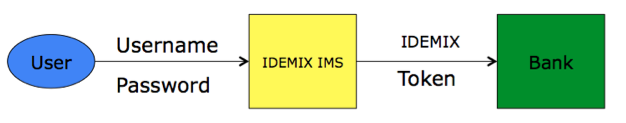
\includegraphics[width=\textwidth]{figures/IDEMIX}
	\caption{Pseudonym System with IDEMIX IMS}
	\label{fig:IDEMIX}
\end{figure}
With the use of IDEMIX IMS we add a pseudonymous layer in the system. This provides us the necessary privacy. In order to do so, IDEMIX IMS just need to store the IDEMIX credential of the user. 
\\The provider doesn’t need to store any mapping database on his side. It is easier for bank to implement, as bank really doesn’t have to trust the IDEMIX IMS to store sensitive data.
\\In case there is a discrepancy, the authorities need to go only to the bank to get the transaction data as well as the mapping data from the IDEMIX tokens.
\section {IDEMIX implementation in the real world}
From above 2 analyses, we conclude that IDEMIX implementation of pseudonymous system is more favorable to bank than the OpenID implementation. 
\\Now we will try to fit this implementation in our system, which includes Nykredit as the Bank, Signicat as the 3rd party, DTU as corporate customer and other government institutions as authorities. 
\section{Summary}
